\chapter{多复变函数}
%应该补充一些复线性空间的线性代数,单独构成一节。
\section{多元全纯函数}
首先快速回顾单复变函数的知识。
我们通常用$\Omg$来表示$\bbC$的开子集,
$z=x+iy$为$\bbC$的坐标。对于$z\in\bbC$以及实数$R>0$,我们令
$$\bbD(z,R):=\{w\in\bbC|\,|w-z|< R\}$$
为以$z$为圆心$R$为半径的开圆盘。

此外,我们有如下常用记号:
$$\left\{\begin{array}{l}
\td z:=\td x + i\td y\\
\td \bar{z} := \td x- i\td y
\end{array}\right.\quad
\left\{\begin{array}{l}
\pp{z}:=\frac{1}{2}
\left(\pp{x}-i\pp{y}\right)\\
\pp{\bar{z}} := \frac{1}{2}
\left(\pp{x}+i\pp{y}\right)
\end{array}\right.
$$
对于函数$f:\Omg\to\bbC$,
称$f$是\textbf{全纯}(holomorphic)的,
\index{holomorphic function\kong 全纯函数}
若在$\Omg$中成立
$$\pbar f:=\pfrac{f}{\bar{z}}\td\zbar=0$$
我们知道,$f$是全纯的当且仅当$f$在$\Omg$
处处能够局部地展开为收敛幂级数。

对于$\bbC$中的紧致集$K$,称函数$f:K\to\bbC$是全纯的,
如果存在$K$的开邻域$\Omg\supseteq K$,
使得$f$可延拓为$\Omg$上的全纯函数。

单复变函数论中有如下重要结果:

\begin{thm}(柯西积分公式)
设$\bbD\subseteq\bbC$为$\bbC$中的开圆盘,$f:\bbD\to\bbC$为
$\bbD$上的全纯函数,且在$\p\bbD$连续,
则对于任意$w\in\bbD$,成立
$$f(w)=\frac{1}{2\pi i}\int_{\p\bbD}\frac{f(z)}{z-w}\td z$$
\end{thm}

此定理能推导出单变量全纯函数理论的“almost everything”.
这里不再赘述。

我们开始考虑多变量全纯函数。

\begin{definition}
设$\Omg\subseteq\bbC^n$为$\bbC^n$的开子集,函数$f:\Omg\to\bbC$
称为(多变量)\textbf{全纯函数},如果满足以下条件:

(1)$f$是连续函数;

(2)对任意$1\leq j\leq n$,以及任意固定的
$z_1,...,z_{j-1};z_{j+1},...,z_n\in\bbC$,关于$z_j$的单变量函数
$$z_j\mapsto f(z_1,...,z_{j-1};z_j;z_{j+1},...,z_n)$$
是(单变量)全纯函数。
\end{definition}

事实上,如果该定义中的(2)成立,那么能推出(1)成立,
也就是说此定义中的(1)可以去掉。其证明比较复杂,我们承认之。

\begin{notation}
对于$\bbC^n$的开子集$\Omg$,我们记
$$\mcalO(\Omg):=\{f:\Omg\to\bbC|f\text{是$\Omg$上的全纯函数}\}$$
\end{notation}
容易知道$\mcalO(\Omg)$有显然的$\bbC$-代数结构。\vs

本节将说明,多变量全纯函数具有一些与单变量全纯函数类似的性质。

\begin{notation}
对于$z=(z_1,z_2,...,z_n)\in\bbC^n$以及$R=(R_1,R_2,...,R_n)\in\bbR^n$,
并且$R_j>0\,\,(\forall 1\leq j\leq n)$,则我们记
$$\bbD(z,R):=\bbD(z_1,R_1)\times\bbD(z_2,R_2)\times
\cdots\times\bbD(z_n,R_n)$$
称为以$z$为中心,$R$为半径的\textbf{多圆柱}(polydisk)。
\index{polydisk\kong 多圆柱}

对于多圆柱$\bbD(z,R)$,我们记
$$\Gamma(z,R):=\p\bbD(z_1,R_1)\times\p\bbD(z_2,R_2)\times
\cdots\times\p\bbD(z_n,R_n)$$
称为$\bbD(z,R)$的\textbf{特征边界}(distinguished boundary)。
\index{distinguished boundary\kong 特征边界}
\end{notation}
特别注意特征边界$\Gamma(z,R)$
并不等于该多圆柱的边界$\p\bbD(z,R)$.

\begin{thm}(多变量全纯函数的柯西积分公式)

设$f:\overline{\bbD(z,R)}\to\bbC$为全纯函数,
则对任意的$w\in\bbD(z,R)$,成立
$$
  f(w)=
       \frac{1}{(2\pi i)^n}\int_{\Gamma(z,R)}
         \frac{f(\xi)\td\xi_1\td\xi_2\cdots\td\xi_n}
              {(\xi_1-w_1)(\xi_2-w_2)\cdots(\xi_n-w_n)}
$$
\end{thm}
\begin{proof}
由多变量全纯函数的定义,
反复使用单变量全纯函数的柯西积分公式即可。这是容易的。
\end{proof}

与单复变函数完全类似,我们也有泰勒展开:

\begin{cor}(多元全纯函数的泰勒展开公式)

对于$f\in\mcalO(\Omg)$,其中$\Omg\subseteq\bbC^n$为开子集,则
对于任何多圆柱$\bbD(z_0,R)$,如果
$\overline{\bbD(z_0,R)}\subseteq\Omg$,则对于任意$w\in\bbD(z_0,R)$,成立
$$
  f(w)=
       \sum_{\afa\in\bbN^n}a_\afa(w-z_0)^\afa
$$
其中
$$
  a_\afa=\frac{1}{(2\pi i)^n}
           \int_{\Gamma(z_0,R)}
             \frac{f(z)}
                  {(z-z_0)^{\afa+1}}
           \td z_1\td z_2\cdots\td z_n
  =\frac{f^{(\afa)}(z_0)}{\afa!}
$$
\label{多元泰勒-cor}
\end{cor}
注意这里的$\afa$为多重指标,即$\afa=(\afa_1,...,\afa_n)$,
其中每个$\afa_i$都为非负整数。
我们记
\begin{eqnarray*}
z^{\afa}&:=&z_1^{\afa_1}z_2^{\afa_2}\cdots z_n^{\afa_n}\\
\afa!&:=&\afa_1!\afa_2!\cdots\afa_n!\\
f^{(\afa)}&:=&(\p_{z_1})^{\afa_1}(\p_{z_2})^{\afa_2}\cdots(\p_{z_n})^{\afa_n}f\\
\afa+1&:=&(\afa_1+1,\afa_2+1,...,\afa_n+1)
\end{eqnarray*}

其中$z=(z_1,...,z_n)\in\bbC^n$,$f$为$n$元全纯函数。
\begin{proof}
与单复变函数的情形完全类似,可由柯西积分公式得到。
\end{proof}

\begin{thm}(柯西不等式)对于$\bbC^n$的开子集$\Omg$,
若$f\in\mcalO(\Omg)$,多圆柱$\overline{\bbD(z_0,R)}\subseteq\Omg$,
则对任意多重指标$\afa\in\bbN^n$,成立
$$\left|f^{(\afa)}(z_0)\right|\leq
\frac{\afa!}{R^\afa}
\sup_{z\in\Gamma(z_0,R)}|f(z)|$$
\end{thm}
\begin{proof}
与单复变函数的情形完全类似。
利用多元泰勒展开(推论\ref{多元泰勒-cor})即可。
\end{proof}

\begin{cor}设$\Omg\subseteq \bbC^n$为\textbf{连通}开集,
$f\in\mcalO(\Omg)$满足$\forall 1\leq k\leq n$,
$\pfrac{f}{z_k}$在$\Omg$上恒为$0$,则$f$在$\Omg$上为常值函数。
\end{cor}

\begin{cor}(刘维尔定理)
设$f\in\mcalO(\bbC^n)$,并且满足
$$|f(z)|\leq A(1+|z|)^B$$
其中$A,B$为正实数,那么$f$必为次数不超过$B$的多项式函数。
\end{cor}

这些性质于单变量全纯函数雷同,证明也是类似的。

\begin{cor}(Montel定理)

设$\Omg$为$\bbC^n$的开子集,则$\mcalO(\Omg)$
中的任何局部一致有界的全纯函数列都存在一致收敛的子列。
\end{cor}
\begin{proof}
仍类似于单复变全纯函数的情形。使用柯西积分公式,再配合
Arzela-Ascoli定理即可。从略。
\end{proof}

现在,简单介绍一些复的微分形式。对于$\bbC^n$,记其复坐标为
$(z_1,z_2,...,z_n)$;视$\bbC^n$为$2n$维实线性空间,
$$z_k=x_k+iy_k$$
从而引入
\begin{eqnarray*}
\td z_k&=&\td x_k+i\td y_k\qquad (1,0)\text{形式}\\
\td \zbar_k&=&\td x_k-i\td y_k\qquad (0,1)\text{形式}
\end{eqnarray*}

\begin{definition}($(p,q)$-形式)

设$\Omg$为$\bbC^n$的非空开集,则形如
$$u(z)=\sum_{|I|=p\atop |J|=q}
a_{IJ}(z)\td z_I\wedge\td\zbar_J$$
的光滑张量场称为$(p,q)$-形式。
记$\Omg$上的$(p,q)$-形式之全体为$C^\infty_{p,q}(\Omg)$.
\end{definition}
这里的$I,J$为多重指标。“光滑”指的是系数函数$a_{IJ}$为$\Omg$上的光滑复值函数。
另外,显然$(0,0)$-形式即为光滑函数;
$C^\infty_{p,q}(\Omg)$具有显然的复线性空间结构,
事实上还是$C^\infty(\Omg)$-模。

\begin{notation}($\pbar$-算子)
定义算子
$$\pbar: C^\infty_{p,q}(\Omg)\to C^\infty_{p,q+1}(\Omg)$$
如下:对于$(p,q)$-形式
$$u:=\sum_{|I|=p\atop|J|=q}
a_{IJ}\td z_I\wedge\td\zbar_J$$
则
$$
  \pbar u=
  \sum_{|I|=p\atop|J|=q}
    \sum_{k=1}^n
      \pfrac{a_{IJ}}{\zbar_k}
      \td \zbar_k\wedge\td z_I\wedge\td\zbar_J
$$
\end{notation}
类似地,也有
$$\p:C_{p,q}^\infty(\Omg)\to C_{p+1,q}^\infty(\Omg)$$
它们与外微分算子$\td$满足关系
$$\td=\p+\pbar$$
由$\td^2=0$,易知
$$\p^2=0,\quad \pbar^2=0,\quad \p\pbar+\pbar\p=0$$

以下事实显然成立:
\begin{lemma}
对于区域$\Omg$上的光滑函数$f\in C^\infty(\Omg)$,
则$f$全纯当且仅当$\pbar f=0$.
\end{lemma}

\begin{rem}(Dolbeault上同调)
对于$\Omg\subseteq\bbC^n$,注意$\pbar^2=0$,
从而对任意$p\geq 0$,有上链复形$C^\infty_{p,\bullet}(\Omg)$:
$$
  \cdots\to
  C^\infty_{p,q-1}(\Omg)
  \xra{\pbar}C^\infty_{p,q}(\Omg)
  \xra{\pbar}C^\infty_{p,q+1}(\Omg)
  \to\cdots
$$
称上同调群
$$H^{p,q}(\Omg):=H^q(C^\infty_{p,\bullet}(\Omg),\pbar)$$
为区域$\Omg$的\textbf{Dolbeault上同调群}。
\index{Dolbeault cohomology}
\end{rem}
类似于外微分$\td$的de-Rham上同调群,
Dolbeault上同调群与$\Omg$的拓扑联系密切。
例如,以下定理十分重要,我们先陈述,以后再证明:

\begin{lemma}(Dolbeault-Grothendieck引理)

设$\bbD\subseteq\bbC^n$为多圆柱,则对于任意$p,q\geq 0$,
$$H^{p,q}(\bbD)=0$$
\end{lemma}

不难发现它与de Rham上同调的Poincare引理有些类似。

\section{解析延拓与Hartogs现象}
上一节介绍了多复变函数的一些“普通的”(与单变量类似)性质,
本节开始介绍多复变函数的一些独特性质。

\begin{lemma}设$f\in C^\infty_c(\bbC)$为复平面上的
紧支光滑函数,则对任意$z\in\bbC$,成立
$$
  \frac{1}{2\pi i}
  \iint_\bbC
    \frac{\p f\big/\p\taubar}
         {\tau-z}
    \td\tau\wedge\td\taubar
=f(z)$$
\end{lemma}
\begin{proof}
基本的微积分练习。考虑换元$\tau=z+re^{i\theta}$,则易知
\begin{eqnarray*}
  \td\tau\wedge\td\taubar&=&-2ir\td r\wedge\td\theta\\
  \pfrac{r}{\taubar}&=&\frac{1}{2}e^{i\theta}\\
  \pfrac{\theta}{\taubar}&=&-\frac{1}{2ir}e^{i\theta}
\end{eqnarray*}
因此有
\begin{eqnarray*}
     \frac{1}{2\pi i}
     \iint_\bbC
       \frac{\p f\big/\p\taubar}
            {\tau-z}
       \td\tau\wedge\td\taubar
&=&
     \frac{-1}{2\pi}
       \int_0^\infty\td r
         \int_0^{2\pi}
           \left(
            -\frac{1}{ir}\pfrac{f}{\theta}(z+re^{i\theta})
           \right)
           \td\theta\\
& &
    +\frac{-1}{2\pi}
     \int_0^{2\pi}\td\theta
       \int_0^\infty
       \left(
         \pfrac{f}{r}(z+re^{i\theta})
       \right)
       \td r\\
&=&
     0+\frac{-1}{2\pi}
     \int_0^{2\pi}
       -f(z)
       \td\theta\\
&=&
     f(z)
\end{eqnarray*}
证毕。
\end{proof}

\begin{lemma}(简单版本的$\pbar$-引理)

设$n\geq 2$,$\fai\in C^\infty_{0,1}(\bbC^n)$
为具有紧支集的光滑$(0,1)$-形式,
且$\pbar\fai=0$,则存在$\bbC^n$上的紧支光滑函数$g$,使得
$$\pbar g=\fai$$
\label{partial-bar引理-简单版本-lemma}
\end{lemma}

\begin{proof}
记光滑$(0,1)$-形式$\fai$为
$$\fai=\sum_{k=1}^n\fai_k(z_1,...,z_n)\td\zbar_k$$
则
\begin{eqnarray*}
     \pbar\fai
&=&
     \sum_{k,l}
       \pfrac{\fai_k}{\zbar_l}
       \td\zbar_l\wedge\td\zbar_k
 =
     \sum_{1\leq l<k\leq n}
       \left(
         \pfrac{\fai_k}{\zbar_l}
        -\pfrac{\fai_l}{\zbar_k}
       \right)
       \td\zbar_l\wedge\td\zbar_k
\end{eqnarray*}
从而由$\pbar\fai=0$可得对任意$k\neq l$,
$$\pfrac{\fai_k}{\zbar_l}=\pfrac{\fai_l}{\zbar_k}$$

考虑如下的$\bbC^n$上的函数$\psi$:对于$z=(z_1,...,z_n)\in\bbC^n$,
$$
  \psi(z)
:=
  \frac{1}{2\pi i}
  \iint_\bbC
    \frac{\fai_1(\tau;z_2,...,z_n)}
         {\tau-z_1}
    \td\tau\wedge\td\taubar
$$
由$\fai_1$的紧支性易知$\psi$为$\bbC^n$上的光滑函数。
对于$1<k\leq n$,有
\begin{eqnarray*}
     \pfrac{\psi(z)}{\zbar_k}
&=&
     \frac{1}{2\pi i}
     \iint_\bbC
       \frac{\pfrac{\fai_1}{\zbar_k}(\tau;z_2,...,z_n)}
            {\tau-z_1}
       \td\tau\wedge\td\taubar\\
&=&
     \frac{1}{2\pi i}
     \iint_\bbC
       \frac{\pfrac{\fai_k}{\taubar}(\tau;z_2,...,z_n)}
            {\tau-z_1}
       \td\tau\wedge\td\taubar\\
&=&
    \fai_k(z)
\end{eqnarray*}
上式对$k=1$显然也成立。因此$\pbar\psi=\fai$.

最后还需要证明$\psi$是紧支的。
由于$\fai$紧支,存在足够大的$R>0$,使得
$$\supp\fai\subseteq \bbD(0,R)$$
因此任意取定$z\in\bbC^n$,使得$z$的分量$z_2,z_3,...,z_n$之中
至少有一个模长大于$R$,则由$\psi$的定义式直接得到$\psi(z)=0$.
(注意:这一步严重依赖$n\geq 2$!)也就是说,存在$z\not\in\bbD(0,R)$
使得$\psi=0$在$z$的某邻域内都成立。
另一方面,由于$\pbar\psi=\fai$且$\supp\fai\subseteq\bbD(0,R)$,
从而$\psi$在$\bbD(0,\bbR)$外部全纯,因此由解析延拓唯一性,
$\psi$在$\bbD(0,R)$外部恒为零,因此$\psi$紧支。
\end{proof}

此引理在单复变$n=1$的情形\textbf{不成立}:
\begin{example}
设$\fai_1\in C_0^\infty(\bbC)$为复平面上的紧支光滑函数,并且
$$\iint_\bbC\fai_1(z)\neq 0$$
考虑$\bbC$上的$(0,1)$-形式$\fai=\fai_1(z)\td\zbar$,
则$\pbar\fai=0$是平凡的,
但\textbf{不存在}紧支光滑函数$\psi$使得$\pbar\psi=\fai$.
\end{example}

\begin{proof}
若存在紧支光滑函数$\psi$使得$\pbar\psi=\fai$,
则$\pfrac{\psi}{\zbar}=\fai_1$.于是
$$
  0\neq
  \iint_\bbC
    \fai_1(z)\td z\wedge\td\zbar
=
  \iint_\bbC
    \pfrac{\psi}{\zbar}
    \td z\wedge\td\zbar
=0
$$
产生矛盾。
\end{proof}

以下是多复变函数解析延拓的令人惊讶的性质,
它与单复变函数有本质不同:

\begin{thm}(Hartogs现象)

设$\Omg\subseteq\bbC^n$为开集$(n\geq 2)$,
$K\ssubset\Omg$且为$\bbC^n$的紧子集,
则对任意的$f\in\mcalO(\Omg\setminus K)$,
都存在解析延拓$F\in\mcalO(\Omg)$,使得
$$F|_{\Omg\setminus K}=f$$
\end{thm}

\begin{proof}
取$K$与$\Omg$直接的截断函数$\psi\in C^\infty_0(\bbC^n)$,
使得$0\leq \psi\leq 1$,
$$K\ssubset\supp\psi\ssubset\Omg$$
并且$\psi|_K\equiv 1$.
考虑$$\ftil:=(1-\psi)f$$
则$\ftil$在整个$\Omg$上都有定义。注意
$$\pbar\ftil=-(\pbar\psi)f+(1-\psi)\pbar f$$
易知$\supp\pbar\ftil\subseteq\supp\psi$.于是由
引理\ref{partial-bar引理-简单版本-lemma},存在光滑函数
$v$,使得$\supp v\subseteq\psi$,并且$\pbar v=\pbar\ftil$,
从而考虑函数
$$F:=(1-\psi)f-v$$
则$\pbar F=0$,从而$F\in\mcalO(\Omg)$.又因为易知
$$F=f\quad(\forall z\in\Omg\setminus\supp\psi)$$
从而由解析延拓唯一性,有$F_{\Omg\setminus K}=f$.
\end{proof}

关于解析延拓,再介绍如下结果:

\begin{lemma}(Hartogs figure)
\index{Hartogs figure}

对于$n>1$,正实数$0\leq r<R$,
以及$\bbC^{n-1}$的开子集$\omg'\subseteq\omg$,
其中$\omg$是连通的。记$\bbC^n$的开子集
$$
  \Omg:=
    \left(
      (\bbD(0,R)\setminus\bbD(0,r))\times\omg
    \right)
    \cup
    \left(
      \bbD(0,R)\times\omg'
    \right)
$$
其中$\bbD(0,r)$与$\bbD(0,R)$
分别为$\bbC$上的以原点为中心,$r,R$为半径的开圆盘。
则任意$f\in\mcalO(\Omg)$都可以(唯一地)解析延拓至
$$\widetilde{\Omg}:=\bbD(0,R)\times\omg$$
\end{lemma}
如此的区域$\Omg$称之为“\textbf{Hartogs figure}”。
$\Omg$的几何图像大致如下:

\begin{figure}[ht]
\centering
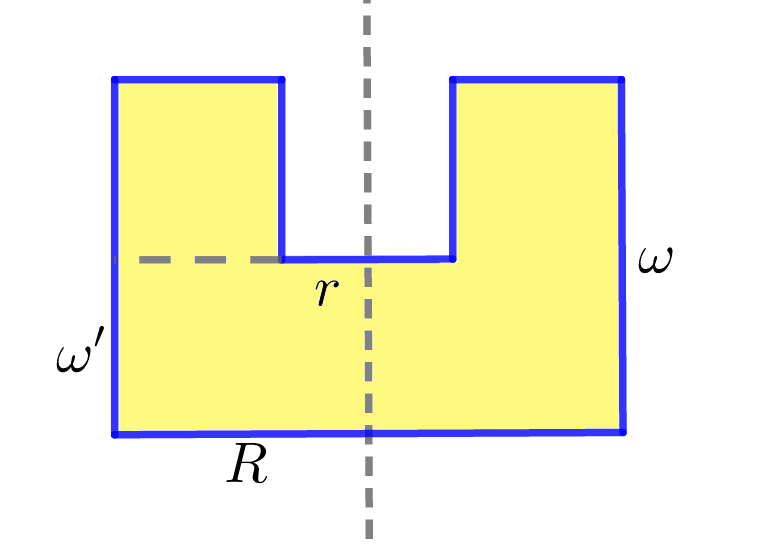
\includegraphics[width=0.4\textwidth]
  {figures/HartogsFigure.png}

图:Hartogs figure示意
\end{figure}

\begin{proof}
容易知道
$$\Omg=\big\{(z_1,\ztil)\in\bbC\times\bbC^{n-1}\big|
r<|z_1|<R,\ztil\in\omg\text{或者}
|z_1|\leq r,\ztil\in\omg'
\big\}$$
对于$f\in\mcalO(\Omg)$,定义$\Omgtil$上的函数
$$
  \ftil(z_1,\ztil):=
    \frac{1}{2\pi i}
    \int_{|w|=\rho}
      \frac{f(w,\ztil)}
           {z_1-w}
      \td w
$$
其中$\rho$为满足$\max\{r,|z_1|\}<\rho<R$的任意实数。
则易知如此定义的$\ftil$为$f$在$\Omgtil$上的解析延拓。
\end{proof}

\begin{thm}(Riemann延拓定理)

考虑$\bbC^n$中的多圆柱$\bbD(0,R)$,其中$n\geq 2$,$R\in\bbR_+^n$。
对任意$2\leq p\leq n$,令$\bbC^n$的子集
$$S:={(z_1,...,z_n)\in\bbC^n|z_1=\cdots=z_p=0}$$
则对任意$f\in\mcalO(\bbD(0,R)\setminus S)$,
$f$都可(唯一地)解析延拓至$\bbD(0,R)$.
\end{thm}

\begin{proof}
这是Hartogs figure的显然推论。记$R=(R_1,R_2,...,R_n)$,
以及$R':=(R_2,...,R_n)\in\bbR^{n-1}$.
考虑$\bbC^{n-1}$的开子集
\begin{eqnarray*}
  \omg &:=&\bbD(0,R')\\
  \omg'&:=&\omg\setminus\{z_2=\cdots=z_p=0\}
\end{eqnarray*}
则易知
$$\bbD(0,R)\setminus S=
\Big(
  \bbD(0,R_1)\setminus\{0\}\times\omg
\Big)
\cup
\Big(
  \bbD(0,R_1)\times\omg'
\Big)
$$
为Hartogs figure,从而完。
\end{proof}

\section{Weierstrass预备定理与除法定理}
回顾单复变函数,若$f$在$0\in\bbC$附近全纯,且$f(0)=0$,
则在$0$附近$f$可以唯一地分解为$f=z^dg(z)$,其中$g$全纯且$g(0)\neq 0$,
$d$为$f$在$0$处的\textbf{零点阶数}。

现在,设$f=f(z,w)$在$0\in\bbC^n(n\geq 2)$附近全纯,
其中$z\in\bbC$,$w\in\bbC^{n-1}$.固定$w$,记
$$f_w(z):= f(z,w)$$
为关于$z$的单复变函数。如果$f_0(0)=0$且$f_0(z)$不恒为零,
则$f_0(z)=z^dg_0(z)$。我们的一个结果是,若“$f_0$”的下标“$0$”稍微“扰动”一下,
则相应的多项式$z^k$也“随之扰动”。

\begin{notation}(Weierstrass 多项式)

对于$(z_0,w_0)\in\bbC\times\bbC^{n-1}$,
则$(z_0,w_0)$处的\textbf{Weierstrass多项式}
是指形如下述的定义于$(z_0,w_0)$附近的$n$元全纯函数:
$$P(z,w)=z^k+a_1(w)z^{k-1}+\cdots+a_k(w)$$
其中$a_i(1\leq i\leq k)$为定义在$w_0\in\bbC^{n-1}$附近的全纯函数,
且$a_i(w_0)=0$.
\index{Weierstrass 多项式}
\end{notation}

关于多元全纯函数在其零点附近的行为,首先有如下:

\begin{thm}(Weierstrass预备定理)

设$f(z,w)$为定义在$(0,0)\in\bbC\times\bbC^{n-1}$附近的全纯函数,
$f(0,0)=0$,且$f_w(z)$在$z=0$附近不恒为零,
则存在唯一的$(0,0)$处的Weierstrass多项式$P(z,w)$,使得
$$f(z,w)=P(z,w)h(z,w)$$
其中$h(z,w)$在$(0,0)$附近全纯,且$h(0,0)\neq 0$.
\end{thm}

\begin{proof}分若干步。

\textbf{Step1}
设$f_0(z)$在$z=0\in\bbC$处的零点阶数为$d\geq 1$,
取足够小的$\veps>0$使得$f_0(z)$在$|z|\leq\veps$之中不再有$z=0$之外的零点。
再由$f$的连续性以及$\{|z|=\veps\}\subseteq\bbC$的紧性,存在足够小的$\veps'>0$,
使得对任意$|z|=\veps,|w|<\veps'$,$f_w(z)\neq 0$.

对于$w\in\bbC^{n-1}$且$|w|<\veps'$,
由辐角原理,$f_w(z)$在$|z|<\veps$内的零点个数(记重数)为
$$
  d(w)=
       \frac{1}{2\pi i}
       \int_{|z|=\veps}
         \frac{f_w'(\xi)}{f_w(\xi)}
         \td\xi
$$
这是关于$w$的连续函数,且$d(0)=d$.从而不妨缩小$\veps'$,使得任意$|w|<\veps'$,
$f_w(z)$在$|z|<\veps$内的零点个数(计重数)均为$d$.

\textbf{Step2}
对于$w\in\bbC^{n-1}$且$|w|<\veps'$,记$f_w(z)$的$d$个零点为
$s_1(w),s_2(w),...,s_d(w)$,它们允许相同,
则$|s_j(w)|<\veps$(注意$s_j(w)$未必为关于$w$的全纯函数)。
特别地$s_1(0)=s_2(0)=\cdots=s_d(0)=0$.
考虑多项式
\begin{eqnarray*}
  P(z,w)&:=&\prod_{j=1}^d(z-s_j(w))\\
         &=&z^d+\sum_{j=1}^da_j(w)z^{d-j}
\end{eqnarray*}
显然系数$a_j(w)$满足$a_j(0)=0$.断言$P(z,w)$为Weierstrass多项式。
为此只需证明$z_j(w)$关于$w$全纯。由代数学可知,系数$a_j$可以写为形如
$s_1^k(w)+s_2^k(w)+\cdots s_d^k(w)\,(k\geq 0)$的$\bbC$-线性组合;
而由留数定理易知
\begin{eqnarray*}
     \sum_{j=1}^ds_j^k(w)
&=&
     \frac{1}{2\pi i}
       \int_{|\xi|=\veps}
         \xi^k
         \frac{f_w'(\xi)}{f_w(\xi)}
         \td\xi
\end{eqnarray*}
从而关于$w$全纯。这就说明了$P(z,w)$的系数函数$a_j(w)$关于$w$全纯。

\textbf{Step3}
令$h(z,w):=\frac{f(z,w)}{P(z,w)}$,断言$h$在$(0,0)$附近全纯,
又因为显然$h(0,0)\neq 0$,从而Weierstrass预备定理的存在性得证。
由单复变易知$h(z,w)$关于$z$全纯,于是只需证明$h$关于$w$全纯。

任取$w\in\bbC^{n-1}$且$|w|<\veps'$,由于$h_w(z):=h(z,w)$关于$z$全纯,从而
$$
  h(z,w)
=
  \frac{1}{2\pi i}
  \int_{|\xi|=\veps}
    \frac{h_w(\xi)}{\xi-z}
    \td\xi
$$
而被积函数$(\xi,w)\mapsto\frac{h_w(\xi)}{\xi-z}$在
$\{(z,w)||z|=\veps,|w|<\veps'\}$的某个邻域全纯,
从而$h(z,w)$关于$w$也全纯。存在性证毕。

\textbf{Step4}
唯一性几乎显然,因为$f$(在$(0,0)$附近)的零点完全由Weierstrass多项式贡献:
对于$w$,以$s_1(w),...,s_d(w)$为零点的关于$z$的首一多项式只能是$P(z,w)$.
\end{proof}

\begin{thm}(Weierstrass除法定理)

设$f(z,w)$为定义在$(0,0)\in\bbC\times\bbC^{n-1}$附近的全纯函数,
$g(z,w)=z^d+\sum\limits_{j=1}^da_j(w)z^{d-j}$为次数为$d$的Weierstrass多项式。
那么存在唯一的$h(z,w)$与$r(z,w)$,
其中$h$为定义在$(0,0)\in\bbC\times\bbC^{n-1}$附近的全纯函数,
$r$为关于$z$的在$(0,0)$处的次数$<d$的多项式,使得
$$f=gh+r$$
在$(0,0)$附近成立。
\end{thm}

\begin{proof}先看唯一性。

\textbf{Step1}
唯一性是容易的。如果$f=gh_1+r_1=gh_2+r_2$,则
$$r_1-r_2=g(h_2-h_1)$$
注意$g,r_1,r_2$为Weierstrass多项式,从而由之前讨论,
存在足够小的$\veps,\veps'>0$使得对任意$w\in\bbC^{n-1}$且$|w|<\veps'$,
$g_w(z)$在$\{|z|<\veps\}$内的零点个数(计重数)恰为$g$的次数$d$,并且
$(r_1-r_2)_w(z)$在此范围内的零点个数(计重数)恰为$(r_1-r_2)$的次数。
注意$r_1,r_2$的次数均小于$d$,从而若$r_1\neq r_2$,
则导致$(r_1-r_2)_w(z)$的零点个数小于$g_w(z)(h_2-h_1)_w(z)$,
因此导致矛盾。这迫使$r_1=r_2$.

\textbf{Step2}
再看存在性。取$\veps,\veps'>0$使得对任意$|z|=\veps$,$|w|\leq\veps'$,
$g_w(z)\neq 0$。对任意$|z|<\veps,|w|<\veps'$,定义
\begin{eqnarray*}
     h(z,w)
 =
     \frac{1}{2\pi i}
     \int_{|\xi|=\veps}
       \frac{f_w(\xi)}
            {g_w(\xi)(\xi-z)}
       \td\xi
\end{eqnarray*}
则易知$h(z,w)$在$(0,0)$附近全纯。再令
$r:=f-gh$,只需证明$r$为关于$z$的次数小于$d$的Weierstrass多项式即可。
事实上,
\begin{eqnarray*}
     r(z,w)
&=&
     f(z,w)-g(z,w)h(z,w)\\
&=&
     \frac{1}{2\pi i}
     \int_{|\xi|=\veps}
       \frac{f_w(\xi)}{\xi-z}
       \td\xi
    -\frac{g_w(z)}{2\pi i}
     \int_{|\xi|=\veps}
       \frac{f_w(\xi)}
            {g_w(\xi)(\xi-z)}
       \td\xi\\
&=&
     \frac{1}{2\pi i}
     \int_{|\xi|=\veps}
       \frac{f_w(\xi)(g_w(\xi)-g_w(z))}
            {g_w(\xi)(\xi-z)}
       \td\xi\\
&=&
     \frac{1}{2\pi i}
     \int_{|\xi|=\veps}
       \frac{f_w(\xi)}{g_w(\xi)}
       \frac{(\xi^d-z^d)+a_1(w)(\xi^{d-1}-z^{d-1})+\cdots}
            {\xi-z}
       \td\xi\\
&=&
     \frac{1}{2\pi i}
     \int_{|\xi|=\veps}
       \frac{f_w(\xi)}{g_w(\xi)}
       \left(
         z^{d-1}+\beta_1(\xi,w)z^{d-2}+\cdots
       \right)
       \td\xi
\end{eqnarray*}
其中函数$\beta_j(\xi,w)$由$g$的系数函数$a_k(w)$决定。
容易看出$r(z,w)$的确为关于$z$的次数$\leq d-1$的多项式。
存在性证毕。
\end{proof}

注意$r$未必是Weierstrass多项式,因为$r(z,w)$的$z^{d-1}$的系数
$$\frac{1}{2\pi i}\int_{|\xi|=\veps}\frac{f_w(\xi)}{g_w(\xi)}\td\xi$$
不见得是$1$(若此积分为$0$,则$r$的首项系数甚至可以是关于$w$的函数)。

\begin{rem}
事实上,Weierstrass除法定理对单复变$n=1$的情形也成立。
设$f(z)=\sum\limits_{k=0}^{\infty}a_kz^k$在$0\in\bbC$附近全纯,
$g(z)=z^d$为次数为$d$的Weierstrass多项式。则令
\begin{eqnarray*}
h(z)&=&\sum_{k=d}^\infty a_kz^{k-d}\\
r(z)&=&\sum_{k=0}^{d-1} a_kz^k
\end{eqnarray*}
则$f=gh+r$满足要求。
\end{rem}

\section{解析函数芽环$\mcalO_{\bbC^n,z}$及其代数结构}

本节继续研究多元解析函数的性质。
首先回顾函数芽的概念。

\begin{definition}(解析函数芽环)

对于$z\in\bbC^n$,记
$$\mcalO_{\bbC^n,z}:=
\{(U,f)|\text{$U$是$z$在$\bbC^n$的一个开邻域,
$f$为定义在$U$上的全纯函数}\}\big/\sim$$
其中模掉的关系$\sim$为
$$(U,f)\sim(V,g)\quad\iff\quad\text{存在$z$的开邻域$W$,
使得$W\subseteq U\cap V$,且$f|_W=g|_W$}$$
\end{definition}
粗俗地说,$\mcalO_{\bbC^n,z}$就是“定义在$z\in\bbC^n$附近的全纯函数之全体”。
之前介绍的Weierstrass预备定理、Weierstrass除法定理其实都是解析函数芽环的性质。
容易验证,$\mcalO_{\bbC^n,z}$在通常的函数加法、乘法下构成\textbf{环}。

我们记$\mcalO_n:=\mcalO_{\bbC^n,0}$.本节介绍环$\mcalO_n$的代数性质。
假定读者熟悉基础的交换代数。本讲义中的“环”默认为含幺、交换的。

\begin{thm}
$\mcalO_n$是局部诺特环($\forall n\geq 1$)。
\end{thm}

回顾:环$A$称为\textbf{局部环}(local ring),
\index{local ring\kong 局部环}
若$A$存在唯一极大理想$\mfkm$
(等价定义:$A$的全体不可逆元构成$A$的理想);
环$A$称为\textbf{诺特环}(Noetherian ring),
\index{Noetherian ring\kong 诺特环}若满足理想升链条件
(等价定义:$A$的每个理想都是有限生成的)。

\begin{proof}
显然$\mcalO_n$为局部环,其极大理想$\mfkm$由定义在$0$附近、在$0$处取值为$0$的函数芽构成。
我们对$n$归纳证明$\mcalO_n$为诺特环。

$n=1$时,在单复变中我们早已熟知$\mcalO_1\cong\{\text{收敛半径$\geq 0$的幂级数}\}$
为主理想整环(PID),其理想形如$J_k=(z^k)$。特别地,为诺特环。

一般地,对于$n\geq 2$,若$\mcalO_{n-1}$为诺特环,
则对$\mcalO_n$的任意非零理想$J$,断言$J$时有限生成的。
任取$0\neq h\in J\subseteq\mfkm$,则$h(0)=0$,不妨$h(z,0)$不恒为零
(其中$z\in\bbC,0\in\bbC^{n-1}$),则由Weierstrass预备定理,
存在Weierstrass多项式$P(z,w)\in\mcalO_{n-1}[z]\subseteq\mcalO_n$
以及函数芽$h'\in\mcalO_n\setminus\mfkm$,
使得$h(z,w)=P(z,w)h'(z,w)$.注意$h'(0,0)$为$\mcalO_n$的可逆元,
又$h\in J$且$J$为$\mcalO_n$的理想,从而$P(z,w)\in J$.

这说明$J$当中必存在Weierstrass多项式。取定
$$P(z,w)=z^d+\sum_{j=1}^{d}a_j(w)z^{d-j}\in J$$
则对任意$f\in J$,对$f,P$使用Weierstrass除法定理,
存在$g(z,w)\in\mcalO_n$,以及
$$r(z,w)=\sum_{k=0}^{d-1}c_k(w)z^k\in\mcalO_{\bbC^{n-1}}[z]$$
为次数至多为$(d-1)$的多项式,使得
$$f=gP+r$$
则$r(z,w)\in J$,并且
容易验证,这诱导了$\mcalO_{n-1}$-模同态
\begin{eqnarray*}
\fai:J &\to    &   \mcalO_{n-1}^{\oplus d}
                   \cong\{r\in\mcalO_{n-1}[z]|\deg_zr<d\}\\
     f &\mapsto&   \sum_{k=0}^{d-1}c_k(w)z^k
\end{eqnarray*}

由归纳假设,$\mcalO_{n-1}$为诺特环,从而$\mcalO_{n-1}^{\oplus d}$
作为有限生成$\mcalO_{n-1}$-模为诺特模,从而其子模$\im \fai$也为有限生成的。
注意$\im\fai\subseteq J$,
记$\{\beta_1,...,\beta_N\}\subseteq\im\fai$
为$\im\fai$的一组$\mcalO_{n-1}$-生成元,其中
$$\beta_j(w)=\sum_{l=0}^{d-1}\beta_{j,l}(w)z^l
\in\mcalO_{n-1}^{\oplus d}$$
则易知
$$\{\beta_j\}_{1\leq j\leq N}\cup \{P(z,w)\}$$
为理想$J$的一组生成元,因此$J$是有限生成的。从而$\mcalO_n$为诺特环。
\end{proof}

\begin{lemma}
设$P,Q\in\mcalO_{n-1}[z]\subseteq\mcalO_n$,
其中$P$为Weierstrass多项式,则$P$整除$Q$在$\mcalO_n$成立,
当且仅当$P$整除$Q$在$\mcalO_{n-1}[z]$中成立。
\label{Weierstrass多项式整除引理-lemma}
\end{lemma}

\begin{proof}
“当”是显然的,只证“仅当”。若$P|Q$在$\mcalO_n$中成立,则令
$$Q(z,w)=f(z,w)P(z,w)$$
其中$f\in\mcalO_n$.另一方面,考虑$\mcalO_{n-1}[z]$中标准的欧几里得带余除法,
$$Q(z,w)=g(z,w)P(z,w)+r(z,w)$$
其中$g,r\in\mcalO_{n-1}[z]$.则Weierstrass除法定理的唯一性迫使
$f=g,r=0$,从而得证。
\end{proof}

\begin{lemma}设$P(z,w)\in\mcalO_{n-1}[z]$为Weierstrass多项式,则:

(1)若在$\mcalO_{n-1}[z]$中有分解
$$P=P_1P_2\cdots P_N$$
则在相差$\mcalO_{n-1}$中的可逆元的意义下,每个$P_j$都为Weierstrass多项式;

(2)$P$为$\mcalO_n$中的不可约元当且仅当$P$为$\mcalO_{n-1}[z]$中的不可约元。
\label{解析函数芽UFD-引理}
\end{lemma}

\begin{proof}$\,$

\textbf{(1)}记$\deg_z P=s$,以及$\deg_z P_j=s_j$,
则$s=\sum\limits_{j=1}^Ns_j$.不妨每个$s_j>0$.考虑$P$的最高次项,有
$$
  z^s=z^s\prod_{j=1}^N\big(\text{$P_j$的$z^{s_j}$系数}\big)
$$
从而相差$\mcalO_{n-1}$中某个可逆元倍,不妨每个$P_j$的$z^{s_j}$系数都为$1$.
再注意
$$z^{s}=P(0,z)=\prod_{j=1}^NP_j(0,z)
=\prod_{j=1}^N(z^{s_j}+\cdots)$$
从而迫使$P_j(0,z)=z^{s_j}$,因此$P_j$为Weierstrass多项式。

\textbf{(2)}“仅当”是显然的,只证“当”。仍记$P(z,w)$关于$z$的次数为$s$.
如果$P$在$\mcalO_n$中可约,令$P=g_1g_2$,其中$g_1,g_2$为$\mcalO_{n}$中的不可逆元,
从而关于$z$的函数$g_1(z,0),g_2(z,0)$在$z=0$处的零点阶数大于$0$,
分别记为$s_1,s_2$.由Weierstrass预备定理,存在分解
$$g_j(z,w)=P_j(z,w)u_j(z,w)\quad (j=1,2)$$
使得$P_j\in\mcalO_{n-1}[z]$为次数为$s_j$的Weierstrass多项式,
$u_j$为$\mcalO_n$中的可逆元。所以在$\mcalO_n$中成立
$(P_1P_2)|P$;再根据引理\ref{Weierstrass多项式整除引理-lemma},可知
$(P_1P_2)|P$在$\mcalO_{n-1}[z]$中也成立。而$P,P_1,P_2$都为首一多项式,
从而必有$P=P_1P_2$,因此$P$在$\mcalO_{n-1}$中可约。
\end{proof}

\begin{thm}
$\mcalO_n$是唯一分解整环(UFD).
\end{thm}

\begin{proof}
对$n$归纳。$n=1$时,$\mcalO_1$为主理想整环,从而为唯一分解整环。
对于$n\geq 2$,如果$\mcalO_{n-1}$为唯一分解整环,则由代数学中的高斯引理,
多项式环$\mcalO_{n-1}[z]$也是唯一分解整环。

现在,对于$\mcalO_n$中的不可逆元$f$,
不妨$z\mapsto f(z,w)|_{w=0}$不恒为零($w\in\bbC^{n-1}$),
从而由Weierstrass预备定理,存在分解$f(z,w)=u(z,w)P(z,w)$,
其中$u$为$\mcalO_n$中的可逆元,$P\in\mcalO_{n-1}[z]$为Weierstrass多项式。
由归纳假设,$\mcalO_{n-1}[z]$为唯一分解整环,从而存在$P$在$\mcalO_{n-1}[z]$
中的分解$P=P_1P_2\cdots P_s$,使得每个$P_j$都为$\mcalO_{n-1}[z]$中的不可约元。
从而由引理\ref{解析函数芽UFD-引理}的(1),不妨每个$P_j$都为Weierstrass多项式;
再对每个$P_j$使用引理\ref{解析函数芽UFD-引理}的(2),知$P_j$为$\mcalO_n$中的不可约元。
从而$f\in\mcalO_n$的不可约分解的存在性证毕。

再看分解的唯一性。只需再证明$\mcalO_n$的不可约元都是素元。
若$f$为$\mcalO_n$中的不可约元,以及$g,h\in\mcalO_n$使得$f|gh$,
断言$f|g$或者$f|h$.由Weierstrass预备定理,
不妨假设$f=f(z,w)$为关于第一个分量$z$的Weierstrass多项式,
从而由$f|gh$知$g(z,0),h(z,0)$也不恒为零,
于是由Weierstrass预备定理也不妨$g,h\in\mcalO_{n-1}[z]$为Weierstrass多项式。
因此$f|gh$在$\mcalO_{n-1}[z]$中成立,而由归纳假设$\mcalO_{n-1}[z]$是唯一分解整环,
且$f$在$\mcalO_{n-1}[z]$不可约,所以$f|g$或者$f|h$在$\mcalO_{n-1}[z]$中成立,
从而在$\mcalO_n$中成立。证毕。
\end{proof}

\section{解析集}
多复变函数与单复变的一个显著区别是解析延拓的难易程度,
Hartogs现象表明多复变函数“更容易被解析延拓”;
而单复变与多复变函数令一个区别是零点集的形态:
在单复变中我们熟知全纯函数零点离散(除非函数恒为零),这在多复变中显然不对,
例如$\bbC^2$上的全纯函数$f(z_1,z_2)=z_1$.

事实上,多元全纯函数的零点集十分重要,
而且是代数几何学中的某些概念(代数簇)的源头。

\begin{definition}(解析集)

设$n\geq 2$, $\bbC^n$的子集$A$称为\textbf{解析集}(analytic set),
\index{analytic set\kong 解析集}
若对任意$z\in A$,存在$z$在$\bbC^n$中的开邻域$\Omg$,
以及$f_1,f_2,...,f_N\in\mcalO(\Omg)$,使得
$$A\cap\Omg=\{w\in\Omg|f_1(w)=f_2(w)=\cdots=f_N(w)\}$$
\end{definition}

也就是说,“局部上看是若干全纯函数的公共零点集”。
对于一个解析集,我们首先局部地研究之——类似于解析函数芽环,我们引入如下概念:

\begin{definition}(解析集芽)对于$x\in\bbC^n$,定义
$$\mcalA_x:=\{(A,x)|x\in A,\,\text{$A$是$\bbC^n$中的解析集}\}/\sim$$
其中关系$\sim$为:$(A_1,x)\sim(A_2,x)\iff$存在$x$在$\bbC^n$中的开邻域
$\Omg$,使得$A_1\cap\Omg=A_2\cap\Omg$.称$\mcalA_x$中的元素为
$x$处的\textbf{解析集芽}。
\end{definition}

$\mcalA_x$中的元素可以认为是包含$x$的“无穷小解析集”。
容易知道它与解析函数芽的关系:任意$(A,x)\in\mcalA_x$,
$(A,x)$为$\mcalO_{\bbC^n,x}$中某些函数的公共零点集。

\begin{definition}对于$x\in\bbC^n$,

(1)对与$x$处的解析集芽$(A,x)\in\mcalA_x$,定义$\mcalO_{\bbC^n,x}$的理想
$$J_{(A,x)}:=\{f\in\mcalO_{\bbC^n,x}|f(z)=0\,\forall z\in A\}$$

(2)对于$\mcalO_{\bbC^n,x}$中的理想$J$,定义$x$处的解析集芽
$$(V(J),x):=\{z\in\bbC^n|g(z)\equiv 0,\,\forall g\in J\}\text{的等价类}$$
\end{definition}
这里并未仔细写清楚,需要验证良定性:注意解析集芽、函数芽实际上都为等价类,
我们需要验证与代表元选取无关,留给读者。

注意$\mcalO_{\bbC^n,x}$为诺特环,从而任何理想$J$都是有限生成的,
记$\{g_1,g_2,...,g_N\}$为其一组生成元,则易知
$$V(J)=\{g_1(x)=g_2(x)=\cdots=g_N(x)=0\}$$
在$x$附近为有限个解析函数的公共零点集,从而的确为解析集(芽)。

\begin{lemma}设$x\in\bbC^n$,$(A,x)\in\mcalA_x$为$x$处的解析集芽,
$J\subseteq\mcalO_{\bbC^n,x}$为理想,则
\begin{eqnarray*}
  J                &\subseteq& J_{(V(J),x)} \\
  (V(J_{(A,x)}),x) &=        & (A,x)
\end{eqnarray*}
\end{lemma}

\begin{proof}
直接按定义验证即可。第一式是容易的;至于第二式,由解析集的定义,$(A,x)$必形如
$$\{g_1(x)=g_2(x)=\cdots=g_N(x)=0\}$$
其中$g_j\in\mcalO_{\bbC^n,x}$,从而$J_{(A,x)}=(g_1,...,g_N)$,
之后容易。
\end{proof}

\begin{rem}不过要注意,第一式的等号未必成立,例如对于$0\in\bbC^2$,
$f(z_1,z_2)=z_1^2$,令$J:=(f)\subseteq\mcalO_{\bbC^2,0}$为由$f$生成的理想,
则$V(J)=\{z_1^2=0\}=\{z_1=0\}$,于是$J_{(V(J),0)}=(z_1)$,
即为由$\ftil(z_1,z_2)=z_1$生成的理想。很明显,$J\varsubsetneqq J_{(V(J),0)}$.
\end{rem}




